\chapter{Results and Discussion}
\label{chap:results}

\section{Overview}
\label{sec:results-overview}

This chapter reports and interprets the benchmark results obtained from the
experimental setup in Chapter~\ref{chap:experimental-setup}.  The European
GBM workload is used as a validation and calibration workload: it verifies
that the framework produces credible Monte Carlo prices and automatic
differentiation outputs against a known Black--Scholes reference.  The main
performance analysis is then carried out on the parametric local-volatility
workload, which is more representative of the target MC+AD setting because
it includes time stepping, a nonlinear volatility surface, and a larger
differentiation graph.

The results combine two layers of evidence. The first layer is a detailed
local CPU study on the Codespace environment, comparing NumPy, JAX/XLA,
C++/OpenMP, and Rust/Rayon where available. This provides the main evidence
for validation, workload scaling, AD overhead, memory pressure, and thread
behaviour. The second layer is the final cloud-profiler study, which adds
Google Cloud cost-performance measurements, Pareto-frontier analysis, and
old-profiler versus SHA selection quality. The discussion below only draws
claims from these measured experiments.

\begin{table}[htbp]
\centering
\footnotesize
\caption{Result sections and their corresponding evidence.}
\label{tab:results-roadmap}
\begin{tabularx}{\textwidth}{p{0.27\textwidth}p{0.28\textwidth}Y}
\toprule
\textbf{Section} &
\textbf{Experiment source} &
\textbf{Main evidence} \\
\midrule
European GBM validation &
European baseline and AD analysis &
Black--Scholes price and Greek agreement used to validate the framework. \\

Local-volatility engine scaling &
LV-1 &
No-AD runtime scaling across NumPy, JAX, C++, and Rust as path count
increases. \\

Local-volatility AD overhead &
LV-2 and LV-4 &
Forward- and reverse-mode JAX AD overhead as a function of path count \(M\)
and time-step count \(N\). \\

Time-step scalability &
LV-3 &
Runtime scaling with the number of local-volatility time steps. \\

Memory and stress limits &
LV-5 and LV-10 &
Resource limits for JAX AD, including observed out-of-memory failures. \\

Thread scalability &
LV-6 and LV-7 &
Strong and weak scaling for C++/OpenMP, Rust/Rayon, and JAX/XLA. \\

Surface-shape sensitivity &
LV-8 &
Runtime effect of changing the local-volatility surface preset. \\

Timing stability &
LV-9 &
Coefficient of variation over 20 repeated runs for key benchmark cells. \\

Final cloud cost-performance &
\code{sha\_cloud\_profiler\_v4} and generated cloud artefacts &
Runtime, estimated cost per run, and best no-AD configurations for priced
cloud instances. \\

Profiler selection quality &
Full-grid, old-profiler, and SHA comparison &
Full runs saved, Pareto recovery, runtime regret, cost regret, rank
correlation, and SHA promotion behaviour. \\
\bottomrule
\end{tabularx}
\end{table}

\section{European GBM Validation}
\label{sec:results-gbm-validation}

The European GBM workload is not the main performance workload in this
chapter.  Its role is to provide a simple analytical reference before
interpreting the more expensive local-volatility experiments.  For the
standard parameter set \(S_0=K=100\), \(r=0.05\), \(\sigma=0.20\), and
\(T=1\), the Black--Scholes analytical call price~\cite{blackscholes1973}
is \(10.4506\), with
Delta \(0.6368\), Vega \(37.524\), and Rho \(53.232\).

\begin{table}[htbp]
\centering
\small
\caption{European GBM baseline validation at \(M=10{,}000\).}
\label{tab:gbm-baseline-validation}
\begin{tabular}{lrrrrr}
\toprule
\textbf{Engine} & \textbf{Price} & \textbf{Mean ms} & \textbf{Std ms}
& \textbf{Paths/s} & \textbf{Rel. price error} \\
\midrule
NumPy/CPU   & 10.3452 & 0.220 & 0.016 & 45.5M  & 1.01\% \\
JAX/XLA     & 10.2098 & 0.559 & 0.051 & 17.9M  & 2.30\% \\
C++/OpenMP  & 10.4658 & 0.098 & 0.009 & 101.6M & 0.15\% \\
\bottomrule
\end{tabular}
\end{table}

The baseline GBM results show that all completed engines produce prices close
to the analytical Black--Scholes value.  The C++ engine is the fastest on
this small single-step workload, achieving \(101.6\) million paths/s, while
NumPy reaches \(45.5\) million paths/s and JAX reaches \(17.9\) million
paths/s.  This result is useful as a sanity check, but it is not treated as
the main performance story because the workload is too small and too simple
to represent the multi-step MC+AD case.

The JAX AD validation also produced accurate Greeks at larger path counts.
At \(M=100{,}000\), forward- and reverse-mode AD gave the same reported
Greek estimates to the displayed precision.  Delta error was \(0.000428\)
(\(0.07\%\)), Vega error was \(0.259\) (\(0.69\%\)), and Rho error was
\(0.080\) (\(0.15\%\)).  This confirms that the JAX AD implementation is
numerically credible before it is used for the local-volatility AD
experiments.

\section{Local-Volatility Smoke Test}
\label{sec:results-lv0}

LV-0 is a smoke test and is not used as a main performance result.  It checks
that each available engine can execute the local-volatility workload and
write results to the shared database.  The test uses only one timed run at
\(M=1{,}000\), so the timings are not statistically meaningful.

\begin{table}[htbp]
\centering
\small
\caption{LV-0: smoke test (\(M=1{,}000\), \(N=252\), one timed run).}
\label{tab:lv0-smoke}
\begin{tabular}{llrrl}
\toprule
\textbf{Engine} & \textbf{AD mode} & \textbf{Latency ms}
& \textbf{Price} & \textbf{Delta / Vega} \\
\midrule
\texttt{cpu}  & none    & 16.000 & 10.61771 & --- \\
\texttt{cpp}  & none    &  7.427 & 10.79929 & --- \\
\texttt{rust} & none    &  5.095 & 12.19688 & --- \\
\texttt{jax}  & none    & 10.205 & 10.33823 & --- \\
\texttt{jax}  & forward & 45.499 & 10.33823 & \(\delta=0.6294,\ \nu=37.49\) \\
\texttt{jax}  & reverse & 23.859 & 10.33823 & \(\delta=0.6294,\ \nu=37.49\) \\
\bottomrule
\end{tabular}
\end{table}

The smoke test confirms that the local-volatility pipeline runs across all
four engines.  The Rust price is visibly different from the other engines at
this very small path count, but this is not interpreted as a correctness
failure because \(M=1{,}000\) is too small for a reliable local-volatility
cross-engine comparison and different engines may use different random
number generators.  The larger \(M\)-sweeps below are used for performance
interpretation.

Because the local-volatility model has no closed-form price, an additional
uncertainty check was run using an independent batched NumPy simulation with
\(M=1{,}000{,}000\), \(N=252\), and seed \(12345\). The discounted payoff
standard deviation from that run was \(14.64743\), giving a Monte Carlo
standard error of \(0.01465\) for the reference price. Table~\ref{tab:localvol-uncertainty}
compares this high-\(M\) reference with the largest LV-1 prices. The
\(z\)-scores use the combined standard error of the reference and the
corresponding \(M=500{,}000\) estimate, using the reference payoff standard
deviation as a common estimate of payoff variance.

\begin{table}[htbp]
\centering
\small
\caption{Local-volatility uncertainty check against an independent batched NumPy reference.}
\label{tab:localvol-uncertainty}
\begin{tabular}{lrrrr}
\toprule
\textbf{Estimate} &
\textbf{\(M\)} &
\textbf{Price} &
\textbf{Difference} &
\textbf{\(z\)-score} \\
\midrule
Independent NumPy reference & \(1{,}000{,}000\) & \(10.44452 \pm 0.01465\) & --- & --- \\
\texttt{cpu} LV-1 & \(500{,}000\) & \(10.47542\) & \(+0.03089\) & \(1.22\) \\
\texttt{cpp} LV-1 & \(500{,}000\) & \(10.46301\) & \(+0.01848\) & \(0.73\) \\
\texttt{jax} LV-1 & \(500{,}000\) & \(10.46082\) & \(+0.01629\) & \(0.64\) \\
\texttt{rust} LV-1 & \(500{,}000\) & \(10.54431\) & \(+0.09979\) & \(3.93\) \\
\bottomrule
\end{tabular}
\end{table}


This check strengthens the numerical interpretation of the local-volatility
results. NumPy, C++ and JAX are within approximately \(1.3\) combined standard
errors of the independent reference, so their price differences are consistent
with Monte Carlo sampling error. The Rust local-volatility price is outside
this range; the discrepancy also persists in the \(M=1{,}000{,}000\) stress
row. For that reason, Rust local-volatility timings are retained as useful
runtime and scaling measurements, but the Rust local-volatility price is not
used as numerical validation evidence. The most likely explanation is the
interaction between Rayon work splitting and per-thread random-number streams,
which should be audited before treating Rust as a trusted local-volatility
pricing backend.

\section{Local-Volatility Engine Scalability}
\label{sec:results-lv1}

LV-1 is the main no-AD engine comparison on the local-volatility workload.
The workload uses \(N=252\) time steps and sweeps path count from
\(10{,}000\) to \(500{,}000\).

\begin{table}[htbp]
\centering
\small
\caption{LV-1: engine scalability on local volatility (\(N=252\), no AD).}
\label{tab:lv1-engine-scalability}
\begin{tabular}{lrrrrrr}
\toprule
\textbf{Engine}
& \textbf{\(M=10k\)}
& \textbf{\(M=25k\)}
& \textbf{\(M=50k\)}
& \textbf{\(M=100k\)}
& \textbf{\(M=250k\)}
& \textbf{\(M=500k\)} \\
& \textbf{ms} & \textbf{ms} & \textbf{ms} & \textbf{ms} & \textbf{ms} & \textbf{ms} \\
\midrule
\texttt{cpu}
& \(100.7\pm 3.5\)
& \(255.8\pm 7.6\)
& \(501.5\pm10.4\)
& \(995.4\pm24.7\)
& \(2448.3\pm25.7\)
& \(5022.4\pm52.0\) \\
\texttt{cpp}
& \(69.8\pm12.9\)
& \(158.8\pm19.2\)
& \(338.6\pm45.4\)
& \(633.4\pm41.8\)
& \(1621.0\pm61.9\)
& \(3062.6\pm82.1\) \\
\texttt{rust}
& \(57.3\pm 9.4\)
& \(122.1\pm11.9\)
& \(239.3\pm14.1\)
& \(497.1\pm32.2\)
& \(1227.7\pm55.0\)
& \(2439.6\pm57.3\) \\
\texttt{jax}
& \(93.4\pm12.6\)
& \(199.6\pm41.4\)
& \(339.3\pm47.8\)
& \(629.9\pm24.2\)
& \(1558.3\pm41.0\)
& \(3103.7\pm45.0\) \\
\bottomrule
\end{tabular}
\end{table}

The local-volatility workload shows approximately linear runtime growth with
path count for all engines.  This is expected because the workload cost is
roughly proportional to \(M\times N\), and \(N\) is fixed at 252 in this
experiment.

Rust/Rayon is the fastest no-AD engine by measured runtime across the full path-count sweep.  At
\(M=500{,}000\), Rust completes the workload in \(2439.6\) ms, compared with
\(3062.6\) ms for C++, \(3103.7\) ms for JAX, and \(5022.4\) ms for NumPy.
This corresponds to approximately \(0.205\) million paths/s for Rust,
\(0.163\) million paths/s for C++, \(0.161\) million paths/s for JAX, and
\(0.100\) million paths/s for NumPy.  Thus, on this local-volatility
workload, Rust is approximately \(2.1\times\) faster than NumPy and about
\(1.25\times\) faster than JAX or C++ at the largest tested path count.

The runtime ranking should be read together with the uncertainty check in
Table~\ref{tab:localvol-uncertainty}. The CPU, C++ and JAX prices are
statistically consistent with the independent high-\(M\) reference, while the
Rust local-volatility price requires further RNG-stream validation. The Rust
local-volatility timings are reported as engineering performance measurements,
but the corresponding prices show a discrepancy relative to the NumPy/JAX/C++
agreement band. Consequently, Rust local-volatility timings should not be
interpreted as evidence of a superior validated pricing engine. They indicate
the performance of the current implementation under the implemented workload,
while correctness requires further investigation.

A notable difference from the simple European GBM workload is that JAX
becomes competitive with C++ on the more expensive multi-step workload.  This
suggests that the fixed overheads of XLA execution are less important once
each benchmark cell contains enough path-level and time-step work.

\section{Local-Volatility AD Scaling with Path Count}
\label{sec:results-lv2}

LV-2 measures the cost of JAX forward- and reverse-mode AD on the
local-volatility workload as the number of paths increases.  All runs use
\(N=252\).

\begin{table}[htbp]
\centering
\small
\caption{LV-2: JAX AD path-count scaling on local volatility (\(N=252\)).}
\label{tab:lv2-ad-m-scaling}
\begin{tabular}{lrrrrr}
\toprule
\textbf{\(M\)}
& \textbf{None ms}
& \textbf{Forward ms}
& \textbf{Reverse ms}
& \textbf{Forward OH}
& \textbf{Reverse OH} \\
\midrule
5k
& \(42.4\pm0.2\)
& \(210.4\pm 4.6\)
& \(90.3\pm 4.9\)
& \(4.94\times\)
& \(2.13\times\) \\
10k
& \(98.8\pm19.8\)
& \(437.0\pm 7.6\)
& \(179.4\pm 5.2\)
& \(5.02\times\)
& \(2.08\times\) \\
25k
& \(166.1\pm20.7\)
& \(985.7\pm51.2\)
& \(373.8\pm14.3\)
& \(6.00\times\)
& \(2.35\times\) \\
50k
& \(340.9\pm40.9\)
& \(1511.3\pm31.9\)
& \(654.6\pm20.5\)
& \(4.87\times\)
& \(2.10\times\) \\
100k
& \(644.1\pm25.8\)
& \(3121.3\pm106.0\)
& \(1312.0\pm35.2\)
& \(4.86\times\)
& \(2.06\times\) \\
250k
& \(1558.2\pm24.0\)
& \(6252.4\pm109.7\)
& \(3627.0\pm82.6\)
& \(4.08\times\)
& \(2.34\times\) \\
\bottomrule
\end{tabular}
\end{table}

The main AD result is clear: reverse-mode AD is substantially cheaper than
forward-mode AD for this scalar-output local-volatility pricing workload.
Across the tested path counts, forward-mode overhead is roughly
\(4.1\)--\(6.0\times\), while reverse-mode overhead is roughly
\(2.1\)--\(2.4\times\).  This is consistent with the expected AD trade-off:
the pricing function has many input parameters but produces a scalar price,
making reverse mode a more suitable differentiation strategy.

The overhead does not vanish at large \(M\).  At \(M=250{,}000\), reverse
mode still costs \(2.34\times\) the no-AD runtime, while forward mode costs
\(4.08\times\).  This shows that AD remains a first-order performance
concern for MC workloads even when the underlying simulation is large enough
to amortise JAX/XLA dispatch overheads.

\section{Local-Volatility Scaling with Time Steps}
\label{sec:results-lv3}

LV-3 separates path-count scaling from time-discretisation scaling by fixing
\(M=50{,}000\) and varying the number of local-volatility time steps.

\begin{table}[htbp]
\centering
\small
\caption{LV-3: time-step scaling on local volatility (\(M=50{,}000\), no AD).}
\label{tab:lv3-n-scaling}
\begin{tabular}{lrrrrr}
\toprule
\textbf{Engine}
& \textbf{\(N=12\)}
& \textbf{\(N=52\)}
& \textbf{\(N=126\)}
& \textbf{\(N=252\)}
& \textbf{\(N=504\)} \\
\midrule
\texttt{cpp}
& \(17.6\pm 5.9\)
& \(66.7\pm 8.3\)
& \(170.2\pm25.7\)
& \(328.0\pm49.3\)
& \(633.2\pm32.2\) \\
\texttt{rust}
& \(12.8\pm 3.1\)
& \(49.9\pm 3.9\)
& \(132.3\pm 7.5\)
& \(256.1\pm18.6\)
& \(519.4\pm63.0\) \\
\texttt{jax}
& \(20.5\pm 3.8\)
& \(61.7\pm 4.8\)
& \(171.4\pm27.3\)
& \(324.0\pm40.8\)
& \(648.7\pm39.5\) \\
\bottomrule
\end{tabular}
\end{table}

Runtime increases approximately linearly with \(N\), which confirms that the
local-volatility workload is dominated by repeated time-step updates rather
than a fixed one-off overhead.  For example, Rust increases from \(256.1\) ms
at \(N=252\) to \(519.4\) ms at \(N=504\), close to a \(2\times\) increase
when the number of time steps doubles.  JAX and C++ show the same general
pattern.

Rust remains the fastest engine by runtime in this experiment, followed by C++ and JAX.
The difference between C++ and JAX is small at \(N=252\), but both are slower
than Rust.  This reinforces the LV-1 result that the Rust/Rayon
implementation is the strongest no-AD local-volatility runtime engine in the
current local environment.

\section{Local-Volatility AD Scaling with Time Steps}
\label{sec:results-lv4}

LV-4 measures how JAX AD overhead changes with the number of time steps.  The
path count is fixed at \(M=25{,}000\).

\begin{table}[htbp]
\centering
\small
\caption{LV-4: JAX AD time-step scaling on local volatility (\(M=25{,}000\)).}
\label{tab:lv4-ad-n-scaling}
\begin{tabular}{lrrrrr}
\toprule
\textbf{\(N\)}
& \textbf{None ms}
& \textbf{Forward ms}
& \textbf{Reverse ms}
& \textbf{Forward OH}
& \textbf{Reverse OH} \\
\midrule
12
& \(7.5\pm0.7\)
& \(50.1\pm 3.5\)
& \(18.6\pm0.8\)
& \(7.14\times\)
& \(2.47\times\) \\
52
& \(28.7\pm0.9\)
& \(203.3\pm 3.8\)
& \(73.9\pm2.2\)
& \(5.11\times\)
& \(2.51\times\) \\
126
& \(72.6\pm2.0\)
& \(504.7\pm27.0\)
& \(186.9\pm9.8\)
& \(6.81\times\)
& \(2.62\times\) \\
252
& \(156.7\pm5.3\)
& \(974.6\pm15.8\)
& \(372.4\pm14.4\)
& \(6.62\times\)
& \(2.52\times\) \\
504
& \(329.5\pm27.7\)
& \(1901.5\pm13.5\)
& \(738.4\pm14.7\)
& \(6.32\times\)
& \(2.33\times\) \\
\bottomrule
\end{tabular}
\end{table}

The AD overhead pattern is stable across simulation length.  Reverse mode
remains close to \(2.3\)--\(2.6\times\) the no-AD runtime, while forward
mode remains much more expensive, usually above \(5\times\).  Increasing the
number of time steps therefore increases absolute runtime for all modes, but
does not change the conclusion that reverse mode is the better AD strategy
for this scalar-output workload.

The \(N=504\) case is particularly important because it doubles the default
daily time-step count.  Even there, reverse mode completes in \(738.4\) ms,
compared with \(1901.5\) ms for forward mode.  This gives a strong practical
argument for reverse-mode AD when many sensitivities are required from a
single price output.

\section{Memory Pressure and Practical Resource Limits}
\label{sec:results-memory}

Memory behaviour is analysed separately because runtime alone does not show
whether a method remains usable at larger \(M\) and \(N\).  This matters
especially for reverse-mode AD, where intermediate values from the scan may
need to be retained or reconstructed during the backward pass.

\begin{table}[htbp]
\centering
\small
\begin{threeparttable}
\caption{LV-5: JAX memory-pressure experiment.}
\label{tab:lv5-memory}
\begin{tabular}{llrrrr}
\toprule
\textbf{\(N\)} & \textbf{AD mode}
& \textbf{\(M=25k\)}
& \textbf{\(M=50k\)}
& \textbf{\(M=100k\)}
& \textbf{\(M=250k\)} \\
& & \textbf{ms} & \textbf{ms} & \textbf{ms} & \textbf{ms} \\
\midrule
\multirow{3}{*}{252}
& none
& \(152.4\pm 5.7\)
& \(315.2\pm23.2\)
& \(650.8\pm38.4\)
& \(1527.9\pm20.5\) \\
& reverse
& \(380.1\pm21.1\)
& \(649.4\pm22.2\)
& \(1332.9\pm64.3\)
& \(3573.5\pm51.4\) \\
& forward
& \(961.8\pm16.9\)
& \(1515.7\pm38.3\)
& \(3103.6\pm62.7\)
& \(6278.7\pm161.8\) \\
\midrule
\multirow{3}{*}{504}
& none
& \(334.5\pm61.9\)
& \(647.6\pm32.6\)
& \(1239.6\pm24.9\)
& \(3102.3\pm58.6\) \\
& reverse
& \(754.8\pm12.3\)
& \(1310.9\pm26.0\)
& \(2595.1\pm78.6\)
& \textsc{oom} \\
& forward
& \(1979.6\pm100.8\)
& \(3006.0\pm49.3\)
& \(6101.9\pm133.7\)
& \(12392.9\pm121.3\) \\
\bottomrule
\end{tabular}
\begin{tablenotes}
\footnotesize
\item \textsc{oom}: the JAX reverse-mode cell at \(M=250k\), \(N=504\)
was killed by the kernel out-of-memory mechanism.
\end{tablenotes}
\end{threeparttable}
\end{table}

The most important memory result is not the small process-level RSS deltas,
which are noisy under JAX/XLA, but the observed out-of-memory boundary.
JAX reverse mode succeeds at \(M=100k\), \(N=504\), but fails at
\(M=250k\), \(N=504\).  It also succeeds at \(M=500k\), \(N=252\) in the
stress test below, but fails at \(M=1M\), \(N=252\).  These failures provide
direct evidence that reverse-mode AD has a practical memory envelope on the
4-core, 16 GB Codespace environment.

Forward mode is slower than reverse mode, but it completes all LV-5 cells,
including \(M=250k\), \(N=504\).  This gives a useful trade-off: reverse
mode is substantially faster for moderate problem sizes, but forward mode may
be more robust in some large memory-stressed settings.

\section{Thread Scalability on Local Volatility}
\label{sec:results-thread-scalability}

LV-6 and LV-7 evaluate CPU thread scaling on the local-volatility workload.
The experiments use requested thread counts \(T=1,2,4\).  C++ and Rust use
explicit OpenMP/Rayon parallelism, while JAX uses XLA's own CPU execution
runtime and is not expected to respond directly to \texttt{OMP\_NUM\_THREADS}.

\subsection{Strong Scaling}
\label{subsec:results-lv6-strong}

\begin{table}[htbp]
\centering
\small
\begin{threeparttable}
\caption{LV-6: strong thread scaling (\(M=100{,}000\), \(N=252\)).}
\label{tab:lv6-strong-scaling}
\begin{tabular}{lrrrrrr}
\toprule
\textbf{Engine}
& \textbf{\(T=1\) ms}
& \textbf{\(T=2\) ms}
& \textbf{\(T=4\) ms}
& \textbf{\(S_2\)}
& \textbf{\(S_4\)}
& \textbf{Efficiency\(_4\)} \\
\midrule
\texttt{cpp}
& \(1944.4\pm37.3\)
& \(973.9\pm5.9\)
& \(629.9\pm31.7\)
& \(2.00\times\)
& \(3.09\times\)
& 77.2\% \\
\texttt{rust}
& \(1787.3\pm2.7\)
& \(900.0\pm4.1\)
& \(488.1\pm34.6\)
& \(1.99\times\)
& \(3.66\times\)
& 91.5\% \\
\texttt{jax}
& \(642.4\pm20.7\)
& \(637.5\pm32.3\)
& \(642.7\pm19.4\)
& \(1.01\times\)
& \(1.00\times\)
& 25.0\% \\
\bottomrule
\end{tabular}
\begin{tablenotes}
\footnotesize
\item \(S_k = T_1/T_k\).  JAX uses XLA's own CPU parallelism and does not
show meaningful sensitivity to the requested OpenMP thread count.
\end{tablenotes}
\end{threeparttable}
\end{table}

C++ and Rust both scale strongly with requested thread count.  Rust improves
from \(1787.3\) ms at one thread to \(488.1\) ms at four threads, giving a
\(3.66\times\) speedup and 91.5\% four-thread efficiency.  C++ improves from
\(1944.4\) ms to \(629.9\) ms, giving a \(3.09\times\) speedup and 77.2\%
efficiency.  This shows that the local-volatility workload exposes
substantial path-level parallelism to compiled CPU engines.

JAX does not scale with the requested thread count in this experiment.  Its
runtime remains close to \(640\) ms for \(T=1,2,4\).  This does not mean JAX
is single-threaded; rather, it suggests that XLA manages CPU parallelism
internally and is not controlled by the same OpenMP/Rayon knobs used by C++
and Rust.

\subsection{Weak Scaling}
\label{subsec:results-lv7-weak}

\begin{table}[htbp]
\centering
\small
\begin{threeparttable}
\caption{LV-7: weak thread scaling (base \(M=50{,}000\) paths/thread, \(N=252\)).}
\label{tab:lv7-weak-scaling}
\begin{tabularx}{\textwidth}{l>{\centering\arraybackslash}X>{\centering\arraybackslash}X>{\centering\arraybackslash}X>{\centering\arraybackslash}X}
\toprule
\textbf{Engine}
& \textbf{\(T=1\), \(M=50k\) ms}
& \textbf{\(T=2\), \(M=100k\) ms}
& \textbf{\(T=4\), \(M=200k\) ms}
& \textbf{TP speedup} \\
\midrule
\texttt{cpp}
& \(961.8\pm 7.6\)
& \(975.2\pm13.8\)
& \(1238.7\pm29.6\)
& \(3.11\times\) \\
\texttt{rust}
& \(893.6\pm 2.1\)
& \(913.4\pm33.7\)
& \(969.9\pm34.2\)
& \(3.68\times\) \\
\texttt{jax}
& \(316.2\pm16.1\)
& \(675.0\pm95.8\)
& \(1252.0\pm32.1\)
& \(1.01\times\) \\
\bottomrule
\end{tabularx}
\begin{tablenotes}
\footnotesize
\item Throughput speedup is computed as
\((4M_{\mathrm{base}}/T_4)/(M_{\mathrm{base}}/T_1)\).  Ideal weak scaling
would give \(4\times\) throughput at approximately constant latency.
\end{tablenotes}
\end{threeparttable}
\end{table}

Weak scaling again favours the compiled engines.  Rust achieves a
\(3.68\times\) throughput speedup from one to four requested threads, while
C++ achieves \(3.11\times\).  Latency is not perfectly constant, especially
for C++ at \(T=4\), but both compiled engines make effective use of
additional requested threads.

JAX shows almost no weak-scaling throughput gain under the requested thread
sweep.  Its latency increases from \(316.2\) ms at \(M=50k\) to \(1252.0\)
ms at \(M=200k\), giving only \(1.01\times\) throughput speedup.  This
supports the interpretation that JAX/XLA's CPU execution strategy is not
controlled by the same explicit thread-count mechanism as the compiled
OpenMP/Rayon engines.

\section{Surface-Shape Sensitivity}
\label{sec:results-surface-sensitivity}

LV-8 tests whether changing the local-volatility surface shape materially
changes runtime.  The experiment compares flat, equity-skew, and
strong-smile presets at \(M=50{,}000\), \(N=252\).

\begin{table}[htbp]
\centering
\small
\begin{threeparttable}
\caption{LV-8: surface-shape sensitivity (\(M=50{,}000\), \(N=252\)).}
\label{tab:lv8-surface-sensitivity}
\begin{tabular}{llrrrr}
\toprule
\textbf{Engine}
& \textbf{AD}
& \textbf{Flat ms}
& \textbf{Equity-skew ms}
& \textbf{Strong-smile ms}
& \textbf{Reverse OH} \\
\midrule
\multirow{2}{*}{\texttt{jax}}
& none
& \(314.9\pm26.8\)
& \(318.1\pm24.6\)
& \(325.5\pm14.8\)
& --- \\
& reverse
& \(669.9\pm47.3\)
& \(663.4\pm27.4\)
& \(682.4\pm77.1\)
& \(2.09\)--\(2.15\times\) \\
\midrule
\texttt{cpp}
& none
& \(347.8\pm64.5\)
& \(327.9\pm14.4\)
& \(341.2\pm75.3\)
& --- \\
\bottomrule
\end{tabular}
\begin{tablenotes}
\footnotesize
\item JAX prices were 10.38974, 10.39082, and 10.40619 for the flat,
equity-skew, and strong-smile presets respectively.  C++ prices were
10.44431, 10.44826, and 10.45843.
\end{tablenotes}
\end{threeparttable}
\end{table}

Surface shape has little effect on runtime.  For JAX no-AD execution, the
three presets all complete between \(314.9\) ms and \(325.5\) ms.  For JAX
reverse mode, overhead remains in a narrow range of \(2.09\)--\(2.15\times\).
This suggests that the cost of the local-volatility workload is dominated by
the number of paths, number of time steps, random number generation, and scan
structure, rather than by the particular parameter values used in the
polynomial volatility surface.

This experiment is still useful because it demonstrates that the framework
can vary model structure while keeping the same execution harness.  That is
important for extensibility: new model presets can be added without changing
the benchmarking methodology.

\section{Timing Stability}
\label{sec:results-timing-stability}

LV-9 repeats selected key cells for 20 timed runs and reports the coefficient
of variation (CV).  This checks whether the benchmark results are stable
enough to support comparisons.

\begin{table}[htbp]
\centering
\small
\begin{threeparttable}
\caption{LV-9: timing stability (\(M=100{,}000\), \(N=252\), 20 timed runs).}
\label{tab:lv9-timing-stability}
\begin{tabular}{llrrrrr}
\toprule
\textbf{Engine}
& \textbf{AD}
& \textbf{Mean ms}
& \textbf{Std ms}
& \textbf{Min ms}
& \textbf{Max ms}
& \textbf{CV} \\
\midrule
\texttt{jax}  & none    & 629.5  & 29.9 & 596.4  & 722.9  & 4.75\% \\
\texttt{jax}  & reverse & 1275.3 & 41.2 & 1227.5 & 1390.2 & 3.23\% \\
\texttt{cpp}  & none    & 632.7  & 43.4 & 594.0  & 739.4  & 6.86\% \\
\texttt{rust} & none    & 486.3  & 22.2 & 459.9  & 529.9  & 4.56\% \\
\bottomrule
\end{tabular}
\begin{tablenotes}
\footnotesize
\item CV \(= \sigma/\mu \times 100\%\).
\end{tablenotes}
\end{threeparttable}
\end{table}

The timing stability experiment shows acceptable variability for a shared
Codespace environment.  CV values range from 3.23\% for JAX reverse mode to
6.86\% for C++.  This is stable enough to support the main engine and AD
comparisons, especially because the observed performance differences between
engines and AD modes are much larger than the measured run-to-run variation.

Rust is both the fastest no-AD engine in this stability subset and one of the
more stable engines, with a CV of 4.56\%.  JAX reverse mode is the most
consistent cell, with a CV of 3.23\%, likely because the compiled execution
path is stable after warmup.

\section{Stress Limit}
\label{sec:results-stress-limit}

LV-10 probes the largest local-volatility workloads attempted on the
Codespace environment.  It compares the fastest compiled no-AD engines
against JAX reverse-mode AD at \(N=252\).

\begin{table}[htbp]
\centering
\small
\begin{threeparttable}
\caption{LV-10: stress limit (\(N=252\), large \(M\)).}
\label{tab:lv10-stress-limit}
\begin{tabular}{llrrr}
\toprule
\textbf{Engine}
& \textbf{AD}
& \textbf{\(M=500k\) ms}
& \textbf{Mem MB}
& \textbf{\(M=1M\) ms} \\
\midrule
\texttt{cpp}  & none    & \(3099.3\pm 41.9\) & ---   & \(6363.0\pm202.2\) \\
\texttt{rust} & none    & \(2422.2\pm 36.7\) & ---   & \(5028.3\pm 36.9\) \\
\texttt{jax}  & reverse & \(6878.3\pm103.9\) & 527.9 & \textsc{oom} \\
\bottomrule
\end{tabular}
\begin{tablenotes}
\footnotesize
\item JAX reverse mode at \(M=1M\), \(N=252\) was killed by the kernel
out-of-memory mechanism.
\end{tablenotes}
\end{threeparttable}
\end{table}

The stress test reinforces two runtime conclusions.  First, Rust remains faster than
C++ at large local-volatility path counts: at \(M=1M\), Rust completes in
\(5028.3\) ms, while C++ takes \(6363.0\) ms.  Second, JAX reverse-mode AD
has a practical memory limit in the current environment.  It completes
\(M=500k\), \(N=252\), but fails at \(M=1M\), \(N=252\).

Together with LV-5, the OOM cases locate the practical JAX reverse-mode
boundary between successful \(M=500k,\ N=252\) and failed \(M=1M,\ N=252\),
and between successful \(M=100k,\ N=504\) and failed \(M=250k,\ N=504\).
This is one of the most important resource-utilisation findings in the
chapter: reverse-mode AD is faster than forward mode for moderate
local-volatility workloads, but memory becomes the limiting factor at larger
path-count/time-step products.

\section{Final Cloud Cost-Performance and Profiler Results}
\label{sec:results-cloud-profiler}

The local experiments above explain the detailed behaviour of the framework on
controlled CPU workloads. The final cloud experiment extends that evidence by
asking whether the framework can make cost-aware benchmark-selection decisions
from stored cloud metadata and cheap probes. The headline experiment is
\code{sha\_cloud\_profiler\_v4}, run at git commit \code{13789b8} on Google
Cloud \code{n2-standard-4} in \code{europe-west1-b}. The full-grid baseline
contains 16 candidate configurations evaluated at three full path counts, for
48 full benchmark cells.

\subsection{Correctness and AD Overhead in the Final Cloud Run}
\label{subsec:cloud-correctness-ad}

The European GBM workload is again used as the analytical validation point.
Table~\ref{tab:correctness-validation} shows the stored JAX AD validation at
\(M=100{,}000\). Forward and reverse mode produce the same reported price and
Greeks in this experiment. The price error is \(0.357\%\), and the absolute
errors for Delta, Vega, and Rho are small relative to the scale of the
reported Greeks.

\begin{table}[htbp]
\centering
\small
\caption{European GBM AD validation against Black--Scholes analytical values at $M=100{,}000$.}
\label{tab:correctness-validation}
\begin{tabular}{lrrrr}
\toprule
\textbf{AD mode} & \textbf{Price err.} & \textbf{Delta err.} & \textbf{Vega err.} & \textbf{Rho err.} \\
\midrule
forward & 0.357\% & 0.000428 & 0.259 & 0.080 \\
reverse & 0.357\% & 0.000428 & 0.259 & 0.080 \\
\bottomrule
\end{tabular}
\end{table}


Table~\ref{tab:ad-overhead} reports JAX AD overhead at \(M=100{,}000\) on
\code{n2-standard-4}. The final cloud results broaden the earlier
local-volatility-only AD discussion by including European, Asian, and
local-volatility workloads in the same cloud comparison.

\begin{table}[htbp]
\centering
\small
\caption{JAX automatic differentiation overhead at $M=100{,}000$ on n2-standard-4.}
\label{tab:ad-overhead}
\begin{tabular}{llrr}
\toprule
\textbf{Workload} & \textbf{AD mode} & \textbf{Runtime ms} & \textbf{Overhead} \\
\midrule
Asian & reverse & 1148.4 & 1.81$\times$ \\
European & forward & 4.783 & 1.96$\times$ \\
European & reverse & 5.208 & 2.10$\times$ \\
Asian & forward & 1552.1 & 2.45$\times$ \\
Local volatility & reverse & 2169.7 & 2.55$\times$ \\
Local volatility & forward & 3768.5 & 4.42$\times$ \\
\bottomrule
\end{tabular}
\end{table}


The measured overheads range from \(1.81\times\) for Asian reverse mode to
\(4.42\times\) for local-volatility forward mode. The ordering is workload
dependent: reverse mode is cheaper than forward mode for the Asian and
local-volatility measurements, while the European forward and reverse overheads
are closer. This reinforces the earlier conclusion that AD mode should be
measured under the actual workload rather than chosen by a fixed rule of
thumb.

\subsection{Cloud Cost-Performance}
\label{subsec:cloud-cost-performance}

Table~\ref{tab:cloud-cost-performance} summarises the best no-AD
cost-performance rows for priced cloud instances at \(M=100{,}000\). Cloud
cost is estimated as marginal compute cost: measured runtime multiplied by the
published or configured hourly instance price. These estimates exclude VM
startup and shutdown time, idle time, storage, orchestration overhead, retries,
network costs, and billing granularity effects. They are therefore suitable for
relative cost-performance comparison under the benchmark protocol, not as exact
end-to-end cloud bills.

\begin{table}[htbp]
\centering
\small
\caption{Best no-AD cost-performance per priced cloud instance at $M=100{,}000$.}
\label{tab:cloud-cost-performance}
\begin{tabularx}{\textwidth}{llYrrr}
\toprule
\textbf{Workload} & \textbf{Instance} & \textbf{Best engine} & \textbf{Runtime ms} & \textbf{Cost/run USD} & \textbf{M paths/s} \\
\midrule
Asian & n2-standard-4 & jax/none & 634.6 & 3.42e-05 & 0.158 \\
Asian & t2d-standard-4 & jax/none & 343.9 & 1.62e-05 & 0.291 \\
European & n2-standard-4 & rust/none & 0.539 & 2.91e-08 & 185.495 \\
European & t2d-standard-4 & rust/none & 0.356 & 1.68e-08 & 281.263 \\
Local volatility & n2-standard-4 & rust/none & 488.9 & 2.64e-05 & 0.205 \\
Local volatility & t2d-standard-4 & rust/none & 443.6 & 2.10e-05 & 0.225 \\
\bottomrule
\end{tabularx}
\end{table}


Figure~\ref{fig:cloud-cost-performance} visualises the same relationship, with
cost per run shown on a logarithmic axis because the absolute marginal compute
costs are small and differ by workload. In the stored priced comparison,
\code{t2d-standard-4} is faster and lower cost per run than
\code{n2-standard-4} for the listed best no-AD workloads. This is an empirical
result for the measured workloads and pricing assumptions, not a claim about
all machine types or future cloud prices.

\begin{figure}[htbp]
    \centering
    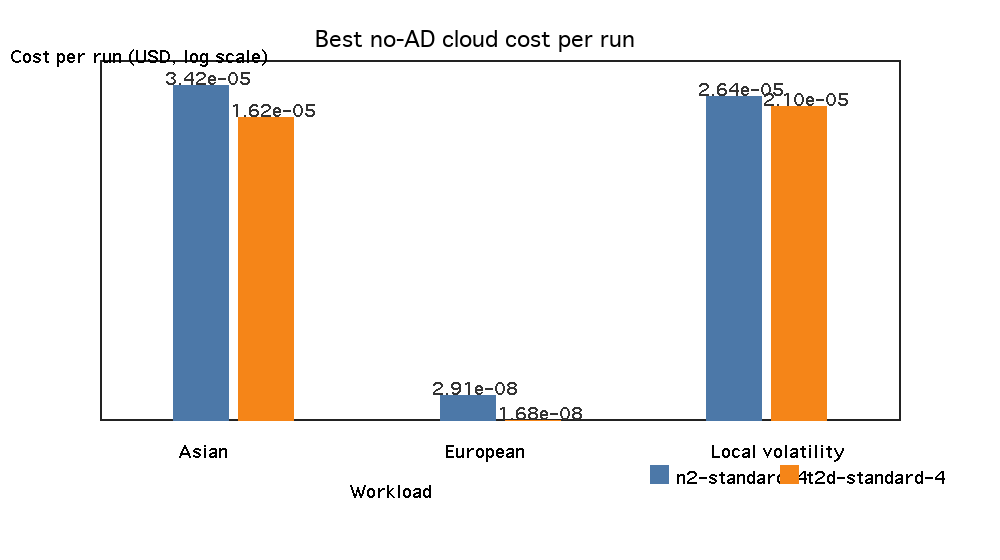
\includegraphics[width=\textwidth]{evaluation/figures/cloud_cost_performance_priced.png}
    \caption{Best no-AD cloud configurations at \(M=100{,}000\). The y-axis uses log-scale marginal compute cost per run; lower-left points indicate faster and cheaper measured configurations under the benchmark protocol.}
    \label{fig:cloud-cost-performance}
\end{figure}

\subsection{Pareto Frontier}
\label{subsec:cloud-pareto}

Figure~\ref{fig:pareto-runtime-cost} plots runtime against estimated cost for
the final \code{n2-standard-4} full-grid comparison. Because the plotted
configurations are on the same instance type, runtime and cost are closely
linked. The value of the Pareto analysis is therefore not that it reveals a
complex two-dimensional trade-off on one machine, but that it gives a precise
target for profiler recovery: a profiler should retain the configurations that
the full grid identifies as non-dominated under the measured metrics.

\begin{figure}[htbp]
    \centering
    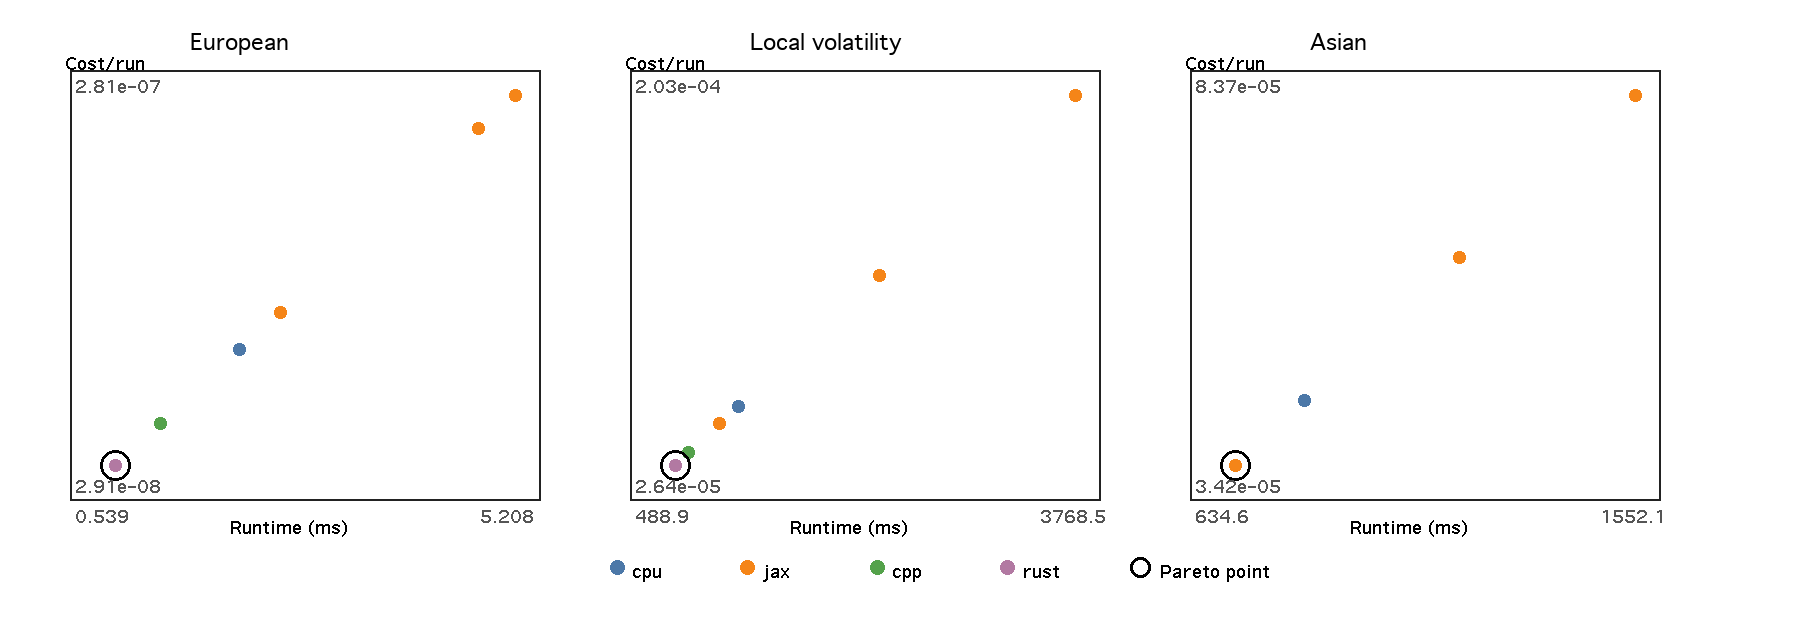
\includegraphics[width=\textwidth]{evaluation/figures/pareto_runtime_cost_n2.png}
    \caption{Runtime versus estimated cost for the final \code{n2-standard-4} grid. Pareto-optimal points are highlighted.}
    \label{fig:pareto-runtime-cost}
\end{figure}

\subsection{Old Profiler versus SHA}
\label{subsec:cloud-profiler-comparison}

Table~\ref{tab:profiler-comparison} is the main final cloud result. The full
grid contains 48 full benchmark runs. The old profiler selects 30 runs, saving
37.5\%. SHA selects 24 runs, saving 50.0\%. Both profilers recover 100.0\% of
the full-grid Pareto frontier and incur 0.0\% runtime and cost regret relative
to the full-grid best. SHA also achieves a stored final probe-to-full Spearman
rank correlation of 1.000, compared with 0.935 for the old profiler evidence.

\begin{table}[htbp]
\centering
\footnotesize
\setlength{\tabcolsep}{4pt}
\renewcommand{\arraystretch}{1.08}
\caption{Full-grid, old-profiler and SHA comparison for the final \code{n2-standard-4} cloud experiment. SHA preserves the full-grid decision on this slice while reducing full-scale runs.}
\label{tab:profiler-comparison}
\begin{tabularx}{\textwidth}{Yrrr}
\toprule
\textbf{Metric} & \textbf{Full grid} & \textbf{Old profiler} & \textbf{SHA} \\
\midrule
Candidate configurations & 16 & 16 & 16 \\
Full benchmark runs & 48 & 30 & 24 \\
Full runs saved & 0 & 18 & 24 \\
Percentage saved & 0.0\% & 37.5\% & 50.0\% \\
Pareto recovery & baseline & 100.0\% & 100.0\% \\
Runtime regret & baseline & +0.0\% & +0.0\% \\
Cost regret & baseline & +0.0\% & +0.0\% \\
Spearman $\rho$ probe--full & -- & 0.935 & 1.000 \\
Probe path-budget saving & -- & -- & 95.5\% \\
Mean scaling-law error & -- & -- & 9.7\% \\
\bottomrule
\end{tabularx}
\end{table}


This result is promising for the \code{n2-standard-4} slice, but it should not
be read as proof that SHA is generally reliable across workloads, instance
families, pricing snapshots, or noisy probe rankings. In the measured headline
grid, SHA halves the number of full-scale cloud benchmark cells while
preserving the full-grid decision quality on the reported metrics. The
practical significance is that the expensive part of the experiment is not
merely shifted elsewhere: the SHA probe path budget is 95.5\% lower than
evaluating the grid at full scale, and the mean scaling-law extrapolation
error is 9.7\%.

\subsection{Guarded SHA Local-Volatility Profiler}
\label{subsec:guarded-sha-localvol}

The robustness issue above motivated a guarded SHA experiment focused on the
local-volatility deployment problem. The candidate space is split into fair
task pools: an all-implemented-backends price-only pool, a validated-backend
price-only pool that excludes Rust because of the local-volatility price
discrepancy discussed in Section~\ref{subsec:limitations-localvol-correctness}, and an
AD-required pool comparing only configurations that produce Greeks. The run
evaluates five four-vCPU Google Cloud instance types
(\code{e2}, \code{n2}, \code{n2d}, \code{c2d}, and \code{t2d}) with \(M=1k\),
\(5k\), and \(25k\) probes and a \(100k\)-path full-grid oracle. The clean
combined artefact contains 120 observations.

\begin{table}[htbp]
\centering
\scriptsize
\caption{Guarded SHA local-volatility recommendations and pure runtime/cost baselines.}
\label{tab:guarded-sha-localvol}
\begin{tabularx}{\textwidth}{l l l l l r}
\toprule
\textbf{Pool/task} & \textbf{Objective} & \textbf{Weighted rec.} & \textbf{Fastest} & \textbf{Cheapest} & \textbf{Regret} \\
\midrule
All price-only & Speed & \code{rust/none/t2d} & \code{rust/none/c2d} & \code{rust/none/t2d} & 0.0\% \\
All price-only & Balanced & \code{rust/none/t2d} & \code{rust/none/c2d} & \code{rust/none/t2d} & 0.0\% \\
All price-only & Cost & \code{rust/none/t2d} & \code{rust/none/c2d} & \code{rust/none/t2d} & 0.0\% \\
Validated price-only & Speed & \code{cpp/none/t2d} & \code{cpp/none/t2d} & \code{cpp/none/t2d} & 0.0\% \\
Validated price-only & Balanced & \code{cpp/none/t2d} & \code{cpp/none/t2d} & \code{cpp/none/t2d} & 0.0\% \\
Validated price-only & Cost & \code{cpp/none/t2d} & \code{cpp/none/t2d} & \code{cpp/none/t2d} & 0.0\% \\
AD-required & Speed & \code{jax/reverse/t2d} & \code{jax/reverse/c2d} & \code{jax/reverse/t2d} & 0.0\% \\
AD-required & Balanced & \code{jax/reverse/t2d} & \code{jax/reverse/c2d} & \code{jax/reverse/t2d} & 0.0\% \\
AD-required & Cost & \code{jax/reverse/t2d} & \code{jax/reverse/c2d} & \code{jax/reverse/t2d} & 0.0\% \\
\bottomrule
\end{tabularx}
\end{table}

\begin{table}[htbp]
\centering
\scriptsize
\caption{Same-grid profiler comparison for the balanced guarded-SHA objective.}
\label{tab:guarded-sha-method-comparison}
\begin{tabularx}{\textwidth}{l r r l r r r l}
\toprule
\textbf{Method} & \textbf{Used} & \textbf{Saved} & \textbf{Selected config.} & \textbf{Obj.} & \textbf{Run} & \textbf{Cost} & \textbf{Validity status} \\
\midrule
Full-grid oracle & 30 & 0 & Price: \code{rust} perf./\code{cpp} valid; AD: \code{jax} & 0.0\% & 0.0\% & 0.0\% & Reference grid \\
Plain SHA & 7 & 23 & Price: \code{rust} perf./\code{cpp} valid; AD: \code{jax} & 0.0\% & 0.0\% & 0.0\% & Less guarded \\
Guarded SHA & 17 & 13 & Price: \code{rust} perf./\code{cpp} valid; AD: \code{jax} & 0.0\% & 0.0\% & 0.0\% & Preferred policy \\
\bottomrule
\end{tabularx}
\end{table}


Table~\ref{tab:guarded-sha-localvol} shows a stronger and more defensible
profiler story than the unguarded SHA audit. The repeated \code{t2d} selection
is not a transcription error: the objective is a weighted runtime--cost score,
not pure elapsed time. \code{c2d} is the fastest pure runtime choice, but
\code{t2d} is only 6.0\% slower and 24.3\% cheaper for price-only, and 4.9\%
slower and 25.5\% cheaper for AD-required. This is enough for \code{t2d} to win
even the speed-sensitive 0.8/0.2 objective.

The all-backend price-only pool selects \code{rust/none/t2d}, but this is a
performance recommendation only. Because Rust local-volatility pricing has not
passed the same cross-engine consistency check as NumPy, C++ and JAX, the
validated price-only deployment recommendation is instead
\code{cpp/none/t2d}. The AD-required recommendation is
\code{jax/reverse/t2d}; these local-volatility sensitivities are internally
consistent JAX AD outputs rather than closed-form-validated Greeks.

The 0.0\% regret values are measured against the observed full-grid oracle for
this tested local-volatility configuration, candidate engines, AD modes,
instance types and \(100k\)-path target budget. They do not imply the true
global optimum over all cloud instances, thread counts, workloads or larger path
budgets. Table~\ref{tab:guarded-sha-method-comparison} shows that plain SHA
also recovers the observed oracle on this grid while selecting fewer full runs;
guarded SHA is reported as the safer policy because it trades some of that
saving for explicit near-tie, engine-diversity, instance-family and
scaling-improvement safeguards. Cloud timing variation means the small
\code{c2d}/\code{t2d} gaps should be interpreted as near-tie deployment
evidence rather than permanent hardware rankings.

\subsection{SHA Progression in the Earlier Multi-Workload Grid}
\label{subsec:sha-progression}

This subsection returns to the earlier multi-workload
\code{sha\_cloud\_profiler\_v4} experiment and visualises the promotion path on
the \code{n2-standard-4} grid. Figure~\ref{fig:sha-progression} shows that all
16 configurations are evaluated at the cheapest probe level, then the active
set is reduced as the path budget increases. The final selected set contains
the configurations promoted for full benchmarking after the profiler's
conservative safeguards are applied.

\begin{figure}[htbp]
    \centering
    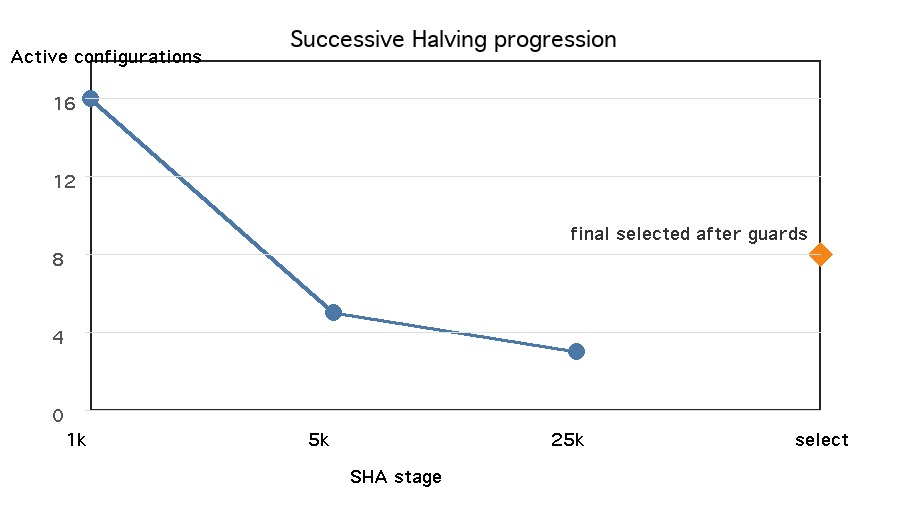
\includegraphics[width=0.95\textwidth]{evaluation/figures/sha_progression_n2.png}
    \caption{SHA promotion path on the earlier \code{n2-standard-4} multi-workload grid. Most configurations receive only cheap probes, while the active set shrinks as the path budget increases.}
    \label{fig:sha-progression}
\end{figure}

The progression illustrates why SHA is useful in this setting. Most
configurations receive only cheap measurements, while promising configurations
receive more budget. In the final experiment this is enough to identify the
same best runtime configuration as the full grid:
\code{rust/european/none} at \(M=100{,}000\), with runtime \(0.54\) ms.

\section{Cross-Question Discussion}
\label{sec:results-discussion}

\subsection{Software Stack and Engine Performance}
\label{subsec:discussion-software-stack}

The local-volatility results show that engine choice has a substantial effect
on throughput.  Rust/Rayon is the fastest no-AD engine by runtime across the main
\(M\)-sweep and the large stress test.  At \(M=500k\), \(N=252\), Rust is
about \(2.1\times\) faster than NumPy and about \(1.25\times\) faster than
JAX or C++.  JAX and C++ are very similar at larger local-volatility sizes,
while NumPy remains consistently slower.

The result also shows why the European GBM workload should not be treated as
the main benchmark.  On the small GBM baseline, C++ was clearly dominant.
On local volatility, Rust becomes fastest and JAX becomes competitive with
C++.  This demonstrates that engine rankings depend strongly on workload
structure.

The numerical interpretation is more cautious. The independent uncertainty
check indicates that NumPy, C++ and JAX agree within estimated Monte Carlo
error on the local-volatility price, while Rust does not. Thus Rust is best
interpreted here as evidence for the throughput available from a Rayon-based
native implementation, not as a fully validated local-volatility pricing
backend.

\subsection{Programming-Language, Runtime and AD-Support Trade-offs}
\label{subsec:discussion-language-ad}

The compiled CPU engines provide the strongest no-AD local-volatility
runtime performance.  Rust/Rayon performs best overall in the local-volatility
timing experiments, while C++/OpenMP remains competitive and scales well with
threads.  JAX/XLA is not the fastest no-AD engine, but it provides the main
AD capability and becomes close to C++ on larger multi-step workloads.

This should not be read as a broad benchmark of AD libraries across languages.
The completed implementation compares JAX forward- and reverse-mode AD against
native no-AD engines in NumPy, C++ and Rust. The C++ and Rust engines are
valuable systems baselines, but they do not evaluate C++ AD tools, Rust AD
libraries, Enzyme, or source-transformation AD in those languages.

The AD results show a clear trade-off.  Reverse-mode AD is consistently much
faster than forward-mode AD for the scalar-output local-volatility pricing
function, with reverse-mode overhead usually around \(2.1\)--\(2.6\times\)
and forward-mode overhead around \(4\)--\(7\times\).  However, reverse mode
also reaches memory limits at larger \(M,N\) combinations.  Therefore, the
best AD choice depends on whether the bottleneck is runtime or memory.

\subsection{Parallelism and Bottlenecks}
\label{subsec:discussion-parallelism}

The thread-scaling results show that C++ and Rust expose path-level
parallelism effectively to OpenMP and Rayon.  Rust achieves \(3.66\times\)
strong-scaling speedup at four requested threads and \(3.68\times\)
weak-scaling throughput speedup.  C++ also scales well, though less strongly,
with \(3.09\times\) strong-scaling speedup and \(3.11\times\) weak-scaling
throughput speedup.

JAX behaves differently.  It is competitive in absolute runtime for no-AD
local-volatility execution, but it does not respond to requested thread-count
changes.  This indicates that XLA's managed CPU runtime should be interpreted
separately from explicit OpenMP/Rayon thread scaling.  For this project, the
main bottlenecks are therefore different by engine: compiled engines are
limited by parallel efficiency and memory bandwidth at higher thread counts,
while JAX is limited by its managed execution model and, for reverse-mode AD,
by memory pressure.

\subsection{Compiler and AD Runtime Techniques}
\label{subsec:discussion-ai-techniques}

The JAX/XLA results provide evidence for the relevance of compiler and AD
runtime techniques to Monte Carlo simulation.  JAX is relatively weak on the
small European GBM baseline, but becomes competitive with C++ on the
multi-step local-volatility workload.  This suggests that XLA-style compiled
execution becomes more attractive when the workload has enough repeated
structure to amortise dispatch and compilation overheads. The conclusion is
therefore limited but useful: in this project, JAX/XLA is most valuable as an
AD-capable compiled backend rather than as a universally fastest no-AD engine.

\subsection{Integrated Scope of the Completed Evaluation}
\label{subsec:discussion-scope}

The completed experiments strongly address local MC+AD benchmarking,
programming-language comparison, AD overhead, memory/resource limits, thread
scalability, and a targeted form of cloud resource selection. The final
cloud-profiler study adds measured cost-performance, Pareto-frontier, and
profiler-selection evidence.

This scope is scientifically useful. The project demonstrates a reproducible
benchmarking framework that can run multiple engines under matched workload
definitions, capture repeated measurements, evaluate AD overheads, reveal
practical resource limits, and attach cloud cost metadata to final selection
decisions. The local-volatility suite also shows that more realistic MC+AD
workloads can change the conclusions drawn from simple one-step baselines.

\section{Limitations and Threats to Validity}
\label{sec:results-limitations}

\subsection{Hardware and Cloud Scope}
\label{subsec:limitations-single-machine}

The detailed scaling and memory experiments were collected on a single
Codespace environment. This makes the comparisons controlled and reproducible
under the recorded conditions, but it prevents broad claims about AMD versus
Intel, workstation versus cloud, or CPU versus GPU performance. The final cloud
experiments add targeted Google Cloud evidence, but those results are still
tied to specific instance types, regions, prices, software versions, and run
dates. They should therefore be interpreted as measured cost-performance
evidence for the reported configurations, not as universal cloud hardware
rankings.

\subsection{Local-Volatility Correctness}
\label{subsec:limitations-localvol-correctness}

The European GBM workload has a closed-form Black--Scholes reference, but
the chosen parametric local-volatility workload does not.  Local-volatility
correctness is therefore assessed through cross-engine consistency and
convergence with larger \(M\), rather than by exact analytical error.  The
additional high-\(M\) uncertainty check quantifies this limitation: NumPy, C++
and JAX agree within estimated Monte Carlo error, while Rust does not. For that
reason, Rust local-volatility results are retained as throughput and scaling
evidence, but Rust is not treated as a correctness-certified local-volatility
pricing backend in the guarded-profiler deployment recommendation. Price
differences between engines may reflect different random-number generators,
path-generation implementations, or, in the Rust case, a backend-specific
issue that requires further investigation. Likely causes include RNG stream
partitioning, per-thread path assignment, discretisation mismatch, or a
payoff/discounting implementation difference. A future validation step should
use deterministic per-path random streams shared across engines and compare
pathwise terminal values before comparing aggregate prices.

The AD correctness story is similarly scoped. European GBM prices and Greeks
are analytically validated against Black--Scholes. Local-volatility prices are
validated by cross-engine agreement and convergence where possible, but
local-volatility Greeks have no closed-form reference in this report. The
reported local-volatility sensitivities are therefore checked as internally
consistent JAX AD outputs, not as analytically validated Greeks. A finite-difference check using common random numbers would be the most useful
next validation step for the reported JAX local-volatility Greeks.

\subsection{Random Number Generation as a Confounder}
\label{subsec:limitations-rng}

The engine comparisons measure complete backend implementations rather than
isolated path-evolution kernels. This is useful for deployment because random
number generation is part of real Monte Carlo runtime, but it also means the
measured differences between NumPy, JAX, C++ and Rust combine simulation-kernel
cost, RNG cost, memory layout, and reduction behaviour. The current results do
not separate these effects. A stronger microbenchmark would run a
pre-generated-normal experiment in which all engines consume the same normal
variates, allowing RNG generation to be separated from path evolution and
payoff reduction.

\subsection{Warm versus Cold JAX Execution}
\label{subsec:limitations-cold-warm}

The main timing tables report warm steady-state runtimes after configured
warmup repetitions. This is appropriate for repeated production-style
simulation and for comparing amortised kernel execution, but it is optimistic
for short-lived cloud jobs where JAX/XLA compilation may be paid on the
critical path. The implementation records and discusses compilation effects,
but the final cloud cost-performance tables do not include a full cold-start
versus warm-start comparison. Therefore, cloud cost claims should be read as
steady-state cost-performance rather than one-off job latency.

\subsection{Cloud Cost Scope}
\label{subsec:limitations-cloud-cost}

The cloud-cost estimates use marginal compute cost only. They intentionally
exclude startup and shutdown time, idle time, persistent storage, orchestration
overhead, retries, network transfer and billing granularity. This is defensible
for comparing measured configurations under the same benchmark protocol, but it
should not be interpreted as an exact Google Cloud invoice or as a complete
end-to-end deployment-cost model.

\subsection{Memory Measurement}
\label{subsec:limitations-memory-measurement}

Process-level memory measurements are coarse, especially for JAX/XLA, which
may cache allocations or materialise intermediates inside compiled execution.
For this reason, small RSS deltas are not over-interpreted.  The OOM events
are treated as stronger evidence than individual low memory-delta readings.

\subsection{Thread Control}
\label{subsec:limitations-thread-control}

Thread-count control is more direct for C++/OpenMP and Rust/Rayon than for
JAX/XLA.  JAX uses its own CPU execution runtime, so requested OpenMP-style
thread counts do not translate into clean JAX scaling experiments.  This is
why JAX thread results are interpreted as runtime behaviour rather than as a
controlled thread-count benchmark.

\section{Summary}
\label{sec:results-summary}

Overall, the results show that MC+AD performance depends on workload structure,
runtime system, differentiation mode, parallel execution model and cloud cost
assumptions. European GBM validates prices and JAX Greeks against
Black--Scholes, while the local-volatility suite exposes the main runtime, AD,
memory and scaling trade-offs. Rust/Rayon gives the fastest measured no-AD
local-volatility timings, but its local-volatility price discrepancy means those
rows are performance evidence rather than correctness evidence. JAX provides the
main AD evidence: reverse mode is faster than forward mode for moderate
scalar-output local-volatility workloads, but reaches memory limits at larger
\(M,N\) combinations.

The cloud results show that marginal cost-performance can differ from raw
runtime ranking. Plain SHA halves full-grid work on the favourable
\code{n2-standard-4} slice, while the guarded local-volatility profiler matches
the observed oracle across the five-instance grid and avoids 13 of 30
full-scale task-level runs. These profiler results are promising, but scoped to
the measured grids and should be read together with the limitations above.
